\documentclass[11pt]{article}

\usepackage[review]{acl}

\usepackage{times}
\usepackage{latexsym}
\usepackage[T1]{fontenc}
\usepackage[utf8]{inputenc}
\usepackage{microtype}
\usepackage{inconsolata}
\usepackage{graphicx}
\usepackage{amsmath}
\usepackage{amssymb}
\usepackage{booktabs}
\usepackage{tipa}
\usepackage{tikz}
\usetikzlibrary{arrows.meta, positioning}

\title{Singable Lyrics Translation with IPA-Augmented LLM Agents}

\author{Anonymous}

\begin{document}
\maketitle

\begin{abstract}
Translating song lyrics while preserving singability requires satisfying musical constraints---syllable counts, rhyme schemes, and syllable patterns---that standard machine translation ignores.
We present a framework that equips a large language model with IPA-based phonetic analysis tools within a ReAct-style agent loop.
The agent extracts constraints from source lyrics, then translates through a multi-phase process, calling tools to iteratively verify and refine each constraint.
We formalize the three musical constraints, describe the IPA tool suite and agent architecture, and propose three evaluation metrics: Syllable Error Rate (SER), Syllable Count Relative Error (SCRE), and Adjusted Rand Index (ARI).
\end{abstract}

\section{Introduction}

A translated song lyric must conform to the musical structure of the original so that it remains \emph{singable} to the same melody \citep{low-2005-pentathlon}.
This requires satisfying hard structural constraints: syllable counts must match melodic phrases, rhyme schemes should be preserved, and word-level syllable distributions should mirror the original phrasing.
Despite theoretical grounding \citep{low-2005-pentathlon,franzon-2008-choices}, computational approaches remain scarce.
Neural MT systems have no mechanism for phonetic constraints, and constrained decoding methods \citep{hokamp-liu-2017-lexically,post-vilar-2018-fast} address lexical but not phonetic constraints.
A fundamental obstacle is that \emph{counting syllables, detecting rhyme, and analyzing phonetic patterns are not tasks that LLMs perform reliably through text generation alone} \citep{gao-etal-2023-pal}.

We address this by equipping an LLM with IPA-based phonetic tools within a ReAct-style agent loop \citep{yao-etal-2023-react}, enabling iterative, constraint-aware translation refinement.
Our framework is open-source and available as a PyPI package for reproducibility and practical use.\footnote{Code and package available at \url{https://github.com/anonymous} (anonymized for review).}

Our contributions are:
\begin{enumerate}
    \item A formalization of three musical constraints---syllable counts, rhyme schemes, and syllable patterns---and IPA-based methods for their extraction and verification (\S\ref{sec:constraints}).
    \item An IPA-augmented tool suite and multi-phase agent loop architecture for constraint-preserving lyrics translation (\S\ref{sec:framework}).
    \item Three automatic evaluation metrics---SER, SCRE, and ARI---designed to measure structural constraint preservation in singable translation (\S\ref{sec:eval}).
\end{enumerate}

\section{Related Work}

\subsection{Song Translation}

\citet{low-2005-pentathlon} proposed treating song translation as a pentathlon balancing singability, sense, naturalness, rhythm, and rhyme, observing that rhythm is often the hardest constraint.
\citet{franzon-2008-choices} identified five translation strategies ranging from adapting lyrics to rewriting both lyrics and melody.
\citet{low-2022-translating} provided an updated theoretical account reinforcing singability as the guiding criterion.

On the computational side, \citet{ou-etal-2023-songs} formalized singable lyric translation as a constrained sequence-to-sequence problem, fine-tuning a neural MT model with length, rhyme, and word boundary constraints for English--Chinese translation.
\citet{guo-etal-2022-automatic} addressed automatic song translation for tonal languages, introducing tonal constraints beyond syllable matching, and \citet{ghazvininejad-etal-2018-neural} tackled neural poetry translation with rhythm and rhyme constraints using constrained decoding.
\citet{ye-etal-2024-sing} proposed quality-aware musical lyrics translation that explicitly models musical features during generation.
\citet{ren-etal-2025-lyricar} introduced a curriculum reinforcement learning framework for controllable lyric translation, balancing multiple constraints through difficulty-aware training.
\citet{zhao-etal-2025-reffly} addressed melody-constrained lyrics editing, directly aligning word-level edits with melodic structure.
\citet{cho-etal-2025-mavl} introduced MAVL, a multilingual audio-video lyrics dataset for animated song translation, providing a benchmark that could facilitate future evaluation of singable translation systems.
These approaches rely on specialized model fine-tuning, constrained decoding, or reinforcement learning; our work instead uses a general-purpose LLM augmented with IPA verification tools in an agent loop, requiring no task-specific training.

\subsection{Constrained Text Generation}

\citet{hokamp-liu-2017-lexically} and \citet{post-vilar-2018-fast} introduced lexically constrained decoding via Grid Beam Search and Dynamic Beam Allocation.
In computational poetry, \citet{ghazvininejad-etal-2016-generating} used finite-state machinery for meter and rhyme, \citet{hopkins-kiela-2017-automatically} generated rhythmic verse with neural networks, and \citet{lau-etal-2018-deep} jointly modeled poetic language, meter, and rhyme.
These approaches enforce constraints at the decoding level or learn them implicitly; ours uses an agent loop where the LLM generates freely but verifies via external tools.

\subsection{Tool-Augmented Language Models}

Recent work has shown that LLMs can be made substantially more capable by giving them access to external tools.
\citet{schick-etal-2023-toolformer} trained language models to autonomously decide when to call tools such as calculators and search engines.
ReAct \citep{yao-etal-2023-react} introduced a paradigm where LLMs alternate between generating reasoning traces and performing actions via external tools, improving performance on tasks requiring grounded, multi-step decision-making.
PAL \citep{gao-etal-2023-pal} demonstrated that offloading computational steps to program execution significantly improves accuracy on reasoning tasks, a finding directly relevant to our use case: syllable counting is a computational task that LLMs perform unreliably but that IPA-based tools handle deterministically.
Chain-of-thought prompting \citep{wei-etal-2022-chain} provides a complementary mechanism for structured reasoning that we combine with tool use in our agent loop.
In machine translation, \citet{jiao-etal-2023-chatgpt} demonstrated that LLMs achieve strong translation quality, but their evaluation did not consider musical or structural constraints.

\subsection{Phonetic Resources}

Our tool suite builds on Phonemizer \citep{bernard-titeux-2021-phonemizer} for text-to-IPA conversion and PanPhon \citep{mortensen-etal-2016-panphon} for phonetic distance computation; both are described in \S\ref{sec:framework}.

\section{Musical Constraints in Lyrics Translation}
\label{sec:constraints}

A singable translation must satisfy three structural constraints, each arising from a different aspect of the relationship between lyrics and melody.
Below we describe each constraint, formalize it, and explain how we extract and verify it using IPA-based analysis.

\subsection{Syllable Count Constraint}
\label{sec:syllable-count}

In sung performance, each syllable maps to one or more musical notes.
When a melody assigns three notes to a phrase, the lyric must contain exactly three syllables---fewer leave notes unmatched, while extra syllables force cramming that disrupts the rhythmic feel.
This makes syllable count the most rigid of the three constraints: rhyme and phrasing mismatches may be tolerable in some styles, but syllable count mismatches are almost always audible.
Formally, given source lyrics $L_s = (l_1, \ldots, l_n)$ in language $\lambda_s$, the constraint requires that translated lyrics $L_t = (l'_1, \ldots, l'_n)$ in target language $\lambda_t$ satisfy $\text{syll}(l'_i, \lambda_t) = \text{syll}(l_i, \lambda_s)$ for all lines $i$.

Syllable counting is language-dependent.
For Chinese, each character constitutes exactly one syllable, so counting is trivial.
For other languages, we convert text to IPA via Phonemizer \citep{bernard-titeux-2021-phonemizer} and count \emph{vowel nuclei}---the vocalic centers of syllables:
\begin{equation}
    \text{syll}(l_i, \lambda_s) = \big|\text{nuclei}\big(\text{IPA}(l_i, \lambda_s)\big)\big|
    \label{eq:syllcount}
\end{equation}
where $\text{nuclei}(\cdot)$ applies a regular expression matching IPA vowels (\textipa{i, I, e, E, \ae, a, A, O, o, U, u, @, 2}, etc.) and diphthong sequences (\textipa{aI, eI, OI, aU, oU}, etc.), with adjacent vowels forming diphthongs counted as single nuclei.
For example, ``\emph{Let it go}'' yields IPA /\textipa{lEt It g@U}/ with three vowel nuclei [\textipa{E}, \textipa{I}, \textipa{@U}], giving a count of 3.
The resulting sequence $\mathbf{s} = (s_1, \ldots, s_n)$ serves as the hard constraint for translation.

\subsection{Rhyme Scheme Constraint}
\label{sec:rhyme-scheme}

Rhyme provides structural cohesion in lyrics, creating sonic expectations that are satisfying when met and jarring when violated.
A song with an $AABB$ scheme feels fundamentally different from one with $ABAB$; preserving the rhyme scheme ensures the translation maintains the same pattern of sonic echoes as the original.
Formally, a rhyme scheme is a labeling $R = (r_1, \ldots, r_n)$ where $r_i \in \{A, B, C, \ldots\}$ assigns each line to a rhyme class, with $r_i = r_j$ if and only if lines $i$ and $j$ rhyme.
The constraint requires that the translation's scheme $R_t$ match the source scheme $R_s$.

We detect rhyme by comparing phonetic endings rather than orthographic forms.
For each line, we extract the \emph{rhyme ending}: the IPA substring from the last vowel nucleus to the end of the transcription.
For Chinese, we extract the pinyin final of the last character instead.
The scheme is constructed by labeling the first line $A$, and assigning each subsequent line the label of any earlier line it rhymes with, or a new label otherwise.
Consider the following example:
\begin{quote}
\small
\emph{The stars shine bright with silver \textbf{light}} $\rightarrow$ /\textipa{laIt}/ $\rightarrow$ ending: /\textipa{aIt}/ \\
\emph{And covers all in purest \textbf{white}} $\rightarrow$ /\textipa{waIt}/ $\rightarrow$ ending: /\textipa{aIt}/ \\
\emph{I stand and watch the world \textbf{below}} $\rightarrow$ /\textipa{bIl@U}/ $\rightarrow$ ending: /\textipa{@U}/ \\
\emph{As gentle winds begin to \textbf{blow}} $\rightarrow$ /\textipa{bl@U}/ $\rightarrow$ ending: /\textipa{@U}/
\end{quote}
Lines 1--2 share ending /\textipa{aIt}/ (class $A$) and lines 3--4 share /\textipa{@U}/ (class $B$), yielding $AABB$.
This IPA-based approach correctly identifies rhymes that orthographic comparison would miss (e.g., ``weight'' and ``late'') and rejects false rhymes based on spelling alone (e.g., ``cough'' and ``through'').

\subsection{Syllable Pattern Constraint}
\label{sec:syllable-pattern}

Even when two lines share the same total syllable count, different word-level distributions create different rhythmic feels.
Consider two eight-syllable lines: ``un-for-get-ta-ble mel-o-dy'' with pattern $[5, 3]$ versus ``I can hear the mu-sic play'' with pattern $[1, 1, 1, 1, 2, 2]$.
The first has two long words producing a flowing feel, while the second has many short words producing a staccato rhythm.
Word boundaries interact with note groupings and breaths in sung performance, so preserving the syllable pattern ensures the translation fits the melody at the phrasing level, not just the syllable level.
Formally, the syllable pattern of a line $l_i$ is a vector $\mathbf{p}_i = (p_{i,1}, \ldots, p_{i,k_i})$ recording the syllable count of each word. The constraint asks that the translation's pattern $\mathbf{p}'_i$ be similar to $\mathbf{p}_i$ while maintaining the same total: $\sum_j p'_{i,j} = \sum_j p_{i,j} = s_i$.

To extract patterns, we apply language-specific word segmentation---space-based tokenization for English and other space-delimited languages, and a neural tokenizer for Chinese---then compute each word's syllable count via Equation~\ref{eq:syllcount}.
We measure pattern similarity using a normalized alignment score.
Given patterns of potentially different lengths, we pad the shorter one with zeros and compute:
\begin{equation}
    \text{sim}(\mathbf{p}, \mathbf{p}') = 1 - \frac{\sum_{j=1}^{m} |p_j - p'_j|}{\sum_{j=1}^{m} \max(p_j, p'_j)}
    \label{eq:patsim}
\end{equation}
where $m = \max(|\mathbf{p}|, |\mathbf{p}'|)$.
A score of 1.0 indicates an exact match; we treat $\geq 0.8$ as acceptable.
For example, ``Let it go'' has pattern $[1, 1, 1]$.
A Chinese translation tokenized as two words with pattern $[2, 1]$ yields $\text{sim}([1,1,1], [2,1,0]) = 0.5$ (poor alignment), whereas a translation tokenized as three single-character words gives pattern $[1, 1, 1]$ with $\text{sim} = 1.0$.

\section{IPA-Augmented Agent Framework}
\label{sec:framework}

We now describe the agent architecture that uses IPA tools to produce constraint-preserving translations.
Figure~\ref{fig:framework} provides an overview of the complete pipeline.

\begin{figure}[t]
\centering
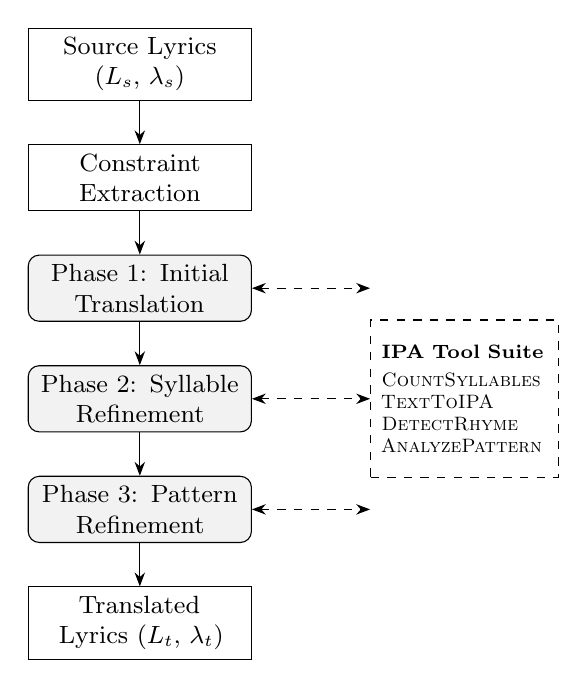
\begin{tikzpicture}[
    node distance=0.55cm and 1.8cm,
    every node/.style={font=\small},
    box/.style={rectangle, draw, text width=2.6cm, minimum height=0.55cm, align=center},
    phase/.style={box, rounded corners, fill=gray!10},
    toolbox/.style={rectangle, draw, dashed, text width=2.1cm, inner sep=4pt, align=left, font=\scriptsize},
    >={Stealth[length=5pt]},
]
\node[box] (src) {Source Lyrics ($L_s$, $\lambda_s$)};
\node[box, below=of src] (ext) {Constraint Extraction};
\node[phase, below=of ext] (p1) {Phase 1: Initial\\Translation};
\node[phase, below=of p1] (p2) {Phase 2: Syllable\\Refinement};
\node[phase, below=of p2] (p3) {Phase 3: Pattern\\Refinement};
\node[box, below=of p3] (out) {Translated Lyrics ($L_t$, $\lambda_t$)};

\node[toolbox, right=1.5cm of p2, minimum height=2.0cm] (tools) {%
\textbf{IPA Tool Suite}\\[2pt]%
\textsc{CountSyllables}\\%
\textsc{TextToIPA}\\%
\textsc{DetectRhyme}\\%
\textsc{AnalyzePattern}};

\draw[->] (src) -- (ext);
\draw[->] (ext) -- (p1);
\draw[->] (p1) -- (p2);
\draw[->] (p2) -- (p3);
\draw[->] (p3) -- (out);
\draw[<->, dashed] (p1.east) -- (tools.west |- p1.east);
\draw[<->, dashed] (p2.east) -- (tools.west);
\draw[<->, dashed] (p3.east) -- (tools.west |- p3.east);
\end{tikzpicture}
\caption{Overview of the IPA-augmented agent framework. Source lyrics undergo constraint extraction, then pass through three refinement phases. Each phase interacts with the IPA tool suite (dashed) via function calls in a ReAct loop.}
\label{fig:framework}
\end{figure}

\subsection{IPA as Universal Phonetic Interface}

The International Phonetic Alphabet provides a standardized, language-independent representation of speech sounds, making it an ideal intermediary for cross-lingual phonetic analysis: regardless of the source or target language, all phonetic operations---syllable counting, rhyme comparison, pattern analysis---can be performed on IPA transcriptions using the same algorithms.
Our system uses Phonemizer \citep{bernard-titeux-2021-phonemizer} as the text-to-IPA backend, wrapping the eSpeak~NG speech synthesizer with support for over 100 languages.
Language codes are normalized internally (e.g., \texttt{zh}, \texttt{zh-cn}, \texttt{cmn} all map to Mandarin Chinese) to provide a uniform interface.
For phonetic distance computation, we use PanPhon \citep{mortensen-etal-2016-panphon}, which maps each IPA segment to a vector of articulatory features, enabling fine-grained similarity measurement.

\subsection{Tool Suite}
\label{sec:tools}

The agent has access to four core IPA-based tools (Table~\ref{tab:tools}), each wrapping a deterministic function that provides capabilities the LLM cannot reliably perform through text generation alone \citep{gao-etal-2023-pal}.

\begin{table}[t]
\centering
\small
\begin{tabular}{@{}lp{4.2cm}@{}}
\toprule
\textbf{Tool} & \textbf{Description} \\
\midrule
\textsc{CountSyllables} & Count syllables via IPA vowel nuclei (or character count for Chinese) \\
\textsc{TextToIPA} & Convert text to IPA transcription via eSpeak~NG \\
\textsc{DetectRhyme} & Detect the rhyme scheme of a set of lines by comparing IPA endings \\
\textsc{AnalyzePattern} & Compare target vs.\ current syllable patterns with structured feedback \\
\bottomrule
\end{tabular}
\caption{Core IPA-based tools available to the agent. All tools accept a language parameter for language-specific processing.}
\label{tab:tools}
\end{table}

\textsc{CountSyllables} is the most frequently called tool: given a text string and language code, it converts to IPA and returns an integer syllable count (\S\ref{sec:syllable-count}).
\textsc{TextToIPA} exposes the raw IPA transcription, allowing the agent to inspect phonetic realizations and reason about which syllables to modify---a form of chain-of-thought reasoning \citep{wei-etal-2022-chain} grounded in phonetic observation.
\textsc{DetectRhyme} analyzes the IPA endings of a set of lines and returns the rhyme scheme (e.g., ``$AABB$''), ensuring judgments are phonetic rather than orthographic.
\textsc{AnalyzePattern} compares a target syllable pattern against the current one, returning the similarity score (Equation~\ref{eq:patsim}), per-word differences, and natural-language suggestions for improvement.
All tools are registered as callable functions via modern LLM function-calling APIs.

\subsection{Constraint Extraction}
\label{sec:extraction}

Before translation begins, the system extracts all three constraints from the source lyrics $L_s$ in language $\lambda_s$: (1) \textbf{syllable counts} $\mathbf{s} = (s_1, \ldots, s_n)$ via \textsc{CountSyllables} on each line, (2) \textbf{rhyme scheme} $R_s$ via \textsc{DetectRhyme} on all lines, and (3) \textbf{syllable patterns} $P_s = (\mathbf{p}_1, \ldots, \mathbf{p}_n)$ via \textsc{AnalyzePattern}.
These constraints are passed to the agent as part of the translation prompt, providing explicit targets for each line.
Table~\ref{tab:constraints-example} shows an example.

\begin{table}[t]
\centering
\small
\begin{tabular}{@{}clcl@{}}
\toprule
\textbf{Line} & \textbf{Text} & \textbf{Syll.} & \textbf{Pattern} \\
\midrule
1 & The snow glows white & 4 & {[1,1,1,1]} \\
2 & On the mountain tonight & 6 & {[1,1,2,2]} \\
3 & Not a footprint to be seen & 7 & {[1,1,2,1,1,1]} \\
4 & A kingdom of isolation & 8 & {[1,2,1,4]} \\
\midrule
\multicolumn{4}{@{}l}{\textbf{Rhyme scheme:} $ABCB$ (\emph{tonight}/\emph{seen} do not rhyme;} \\
\multicolumn{4}{@{}l}{\quad detected via IPA ending comparison)} \\
\bottomrule
\end{tabular}
\caption{Example constraint extraction from English source lyrics. Syllable counts are computed via IPA vowel nuclei; patterns via space-based word segmentation.}
\label{tab:constraints-example}
\end{table}

\subsection{Multi-Phase Agent Loop}
\label{sec:loop}

Translation proceeds through three phases, implemented as a directed acyclic graph where each node represents a processing step and conditional edges encode control flow.
The design reflects the priority ordering identified by \citet{low-2005-pentathlon}: semantic content and rhythm (syllable counts) take precedence, followed by phrasing (patterns), with rhyme considered throughout but given lower priority.

\paragraph{Phase 1: Initial Translation with Tool-Guided Reasoning.}
The agent receives a structured prompt containing the source lyrics, target language, and all extracted constraints.
It generates an initial translation of all lines, following a ReAct loop \citep{yao-etal-2023-react}: the LLM generates reasoning about how to satisfy constraints, calls tools to verify its output, observes the results, and adjusts within the same generation turn.
The prompt instructs the agent to consider all three constraints simultaneously, producing a ``best-effort'' initial translation.

A typical interaction proceeds as: the agent reasons about the target syllable count for a line, drafts a translation, calls \textsc{CountSyllables} to verify, observes the result, and adjusts if needed---continuing until all lines are translated.

\paragraph{Phase 2: Line-by-Line Syllable Refinement.}
The initial translation rarely satisfies all syllable constraints exactly.
In this phase, the agent processes each line individually, computing the actual syllable count and comparing it to the target.
If there is a mismatch, the agent receives explicit feedback (e.g., ``Line $i$ has $s'_i$ syllables but the target is $s_i$; please revise while preserving meaning'') and generates a revised translation.
The system re-checks via \textsc{CountSyllables}, continuing for up to 10 iterations; if no exact match is found, the closest attempt is retained.
This phase is critical because even a single syllable mismatch can make a line unsingable.

\paragraph{Phase 3: Syllable Pattern Refinement.}
After syllable counts are matched, the agent refines word-level syllable distributions.
For each line, \textsc{AnalyzePattern} compares the current pattern against the target and returns structured feedback including the similarity score, per-word differences, and suggestions (e.g., ``split the first word into shorter components'').
The agent generates up to three alternative translations per line and selects the one with the highest pattern similarity, subject to maintaining the correct total syllable count.
Lines already achieving similarity $\geq 0.8$ are left unchanged.

\paragraph{Priority and termination.}
The three-phase design addresses constraints in order of importance: syllable counts first (hardest constraint), then syllable patterns.
Rhyme is monitored throughout Phases 1 and 2 via \textsc{DetectRhyme}, but is not given a dedicated refinement phase because rhyme violations are generally less disruptive to singability than syllable mismatches \citep{low-2005-pentathlon}.
The process terminates after Phase 3 with a final validation step.

\subsection{Worked Example}

To illustrate, consider translating ``\emph{Not a footprint to be seen}'' (7 syllables, pattern $[1, 1, 2, 1, 1, 1]$) into Chinese.
In Phase~1, the agent produces a 7-character translation; syllable counting confirms the match, so Phase~2 skips this line.
In Phase~3, pattern analysis reveals the Chinese tokenization yields $[3, 2, 2]$---similarity 0.38 against the target---and suggests splitting the first word.
The agent revises to a translation with single-character tokenization, yielding $[1, 1, 1, 1, 1, 1, 1]$ and similarity 0.71: an improvement, though not exact.
This illustrates a fundamental challenge---Chinese word boundaries are determined by semantics and do not always permit arbitrary decomposition.

\section{Evaluation Metrics}
\label{sec:eval}

Standard MT metrics such as BLEU measure n-gram overlap and do not capture whether a translation preserves musical structure.
We propose three complementary metrics, each targeting one of the three musical constraints.

\subsection{Syllable Error Rate (SER)}

SER measures the overall alignment between the source and translated syllable count sequences using the Levenshtein edit distance \citep{levenshtein-1966}:
\begin{equation}
    \text{SER} = \frac{\text{Lev}(\mathbf{s}, \mathbf{s}')}{\max(|\mathbf{s}|, |\mathbf{s}'|)}
\end{equation}
where $\mathbf{s} = (s_1, \ldots, s_n)$ and $\mathbf{s}' = (s'_1, \ldots, s'_m)$ are the source and translated syllable count sequences, and $\text{Lev}$ operates over sequences of integers (with substitution cost equal to 1 regardless of the magnitude of the difference).

SER captures both \emph{substitution errors} (a line has the wrong syllable count) and \emph{structural errors} (lines are missing or added).
$\text{SER} = 0$ indicates perfect preservation; higher values indicate greater divergence.
Unlike per-line metrics, SER penalizes translations that drop or add lines, which is important because line structure directly corresponds to melodic phrases.

\subsection{Syllable Count Relative Error (SCRE)}

SCRE provides a normalized, per-line view of syllable accuracy, assuming the translation preserves the number of lines ($m = n$):
\begin{equation}
    \text{SCRE} = \frac{1}{n} \sum_{i=1}^{n} \frac{|s_i - s'_i|}{s_i}
\end{equation}

SCRE weights errors relative to line length: a two-syllable error on a four-syllable line ($\text{SCRE}_i = 0.5$) is penalized more heavily than on a twelve-syllable line ($\text{SCRE}_i = 0.17$).
This reflects the intuition that short lines leave less room for syllabic deviation---a single extra syllable in a three-syllable phrase is far more noticeable than in a long verse.
$\text{SCRE} = 0$ indicates all lines match exactly.

SER and SCRE are complementary: SER captures structural alignment including line count mismatches, while SCRE provides percentage-based accuracy that is more interpretable for line-by-line comparison.

\subsection{Adjusted Rand Index (ARI)}

To measure rhyme scheme preservation, we treat the rhyme scheme as a \emph{clustering} of lines and compute the Adjusted Rand Index \citep{hubert-arabie-1985} between the source and translated clusterings.

Let $R_s = (r_1, \ldots, r_n)$ and $R_t = (r'_1, \ldots, r'_n)$ be the rhyme scheme labelings.
The Rand Index (RI) counts the fraction of line pairs that are either in the same cluster in both schemes or in different clusters in both schemes.
ARI adjusts RI for the expected value under random label assignments:
\begin{equation}
    \text{ARI} = \frac{\text{RI} - \mathbb{E}[\text{RI}]}{\max(\text{RI}) - \mathbb{E}[\text{RI}]}
\end{equation}

ARI $\in [-1, 1]$: $1$ indicates the translation perfectly preserves the rhyme structure, $0$ indicates chance-level agreement, and negative values indicate systematic disagreement.
Crucially, ARI is robust to label permutation---a source with scheme $AABB$ and a translation with $BBAA$ receives $\text{ARI} = 1$, since the grouping structure is identical.

Together, SER, SCRE, and ARI cover the structural dimensions of singable translation.
They deliberately do not measure semantic fidelity or naturalness; we view them as complementary to standard MT metrics such as BLEU and COMET.
A good singable translation should score well on both semantic quality metrics and structural quality metrics---high BLEU with high SER would indicate a good translation that is unsingable, while low SER with low BLEU would be structurally correct but semantically wrong.

\section{Experiments}
\label{sec:experiments}

We conduct preliminary experiments to evaluate the effectiveness of IPA-augmented tool use for constraint-preserving lyrics translation.

\subsection{Setup}

We evaluate on English--Chinese song translation in both directions: English-to-Chinese ($\text{en} \rightarrow \text{cmn}$) and Chinese-to-English ($\text{cmn} \rightarrow \text{en}$).
Our test set consists of 500 popular songs covering both English and Chinese tracks across pop, ballad, and rock genres.
Each test case uses 4--20 lines from a song, with lines filtered to contain only the source language.

\paragraph{Implementation.}
The agent framework is implemented using LangGraph, which provides a graph-based orchestration layer for defining the multi-phase agent loop described in \S\ref{sec:loop}.
Each phase is represented as a node in a directed graph with conditional edges encoding the control flow between constraint extraction, initial translation, syllable refinement, and pattern refinement.
For LLM inference, we use Qwen3-30B (4-bit quantized) served locally via Ollama, which provides an OpenAI-compatible API for function calling.
The IPA tools (\S\ref{sec:tools}) are registered as callable functions through LangGraph's tool-binding interface, enabling the ReAct-style reasoning-and-acting loop.

\paragraph{Conditions.}
We compare two conditions using the same underlying model:
\begin{itemize}
    \item \textbf{Base LLM}: Direct translation via Qwen3-30B with a prompt requesting syllable-count preservation, but \emph{without} access to IPA tools or iterative refinement.
    \item \textbf{BLT Agent}: Our full framework with IPA tool suite and multi-phase refinement loop (Phases 1--3 as described in \S\ref{sec:loop}), orchestrated by LangGraph.
\end{itemize}
Both conditions use the same model, isolating the effect of tool-augmented iterative refinement.
We report SER and SCRE as defined in \S\ref{sec:eval}; ARI evaluation requires longer passages with richer rhyme structure and is reserved for future work.

\subsection{Overall Results}

Table~\ref{tab:overall} presents the aggregate results across both translation directions.

\begin{table}[t]
\centering
\begin{tabular}{@{}lcc@{}}
\toprule
\textbf{Method} & \textbf{SER} $\downarrow$ & \textbf{SCRE} $\downarrow$ \\
\midrule
Base LLM   & 0.8729 & 1.2756 \\
BLT Agent  & \textbf{0.5970} & \textbf{0.4499} \\
\bottomrule
\end{tabular}
\caption{Overall results aggregated across both translation directions. Lower is better for both metrics. Bold indicates the best result.}
\label{tab:overall}
\end{table}

The BLT Agent substantially outperforms the Base LLM on both metrics.
SER decreases from 0.8729 to 0.5970 (31.6\% relative reduction), indicating that the tool-augmented agent produces syllable count sequences much closer to the source.
The improvement on SCRE is even more pronounced: a reduction from 1.2756 to 0.4499 (64.7\% relative reduction).
A Base LLM SCRE of 1.2756 means that, on average, each line deviates from the target syllable count by more than 100\% relative to the target---effectively, the baseline pays little attention to syllable constraints.
The BLT Agent reduces this to 0.4499, still imperfect but representing a meaningful step toward singable translation.

\subsection{Per-Language-Pair Results}

Table~\ref{tab:perpair} breaks down performance by translation direction, revealing an asymmetry between the two directions.

\begin{table}[t]
\centering
\begin{tabular}{@{}lcccc@{}}
\toprule
 & \multicolumn{2}{c}{\textbf{SER} $\downarrow$} & \multicolumn{2}{c}{\textbf{SCRE} $\downarrow$} \\
\cmidrule(lr){2-3} \cmidrule(lr){4-5}
\textbf{Pair} & Agent & Base & Agent & Base \\
\midrule
$\text{en} \rightarrow \text{cmn}$ & \textbf{0.238} & 0.810 & \textbf{0.085} & 0.250 \\
$\text{cmn} \rightarrow \text{en}$ & \textbf{0.577} & 0.811 & 0.258 & \textbf{0.246} \\
\bottomrule
\end{tabular}
\caption{Per-language-pair results. Bold indicates the best result for each metric and direction.}
\label{tab:perpair}
\end{table}

\paragraph{English-to-Chinese.}
The $\text{en} \rightarrow \text{cmn}$ direction shows the strongest improvements.
SER drops from 0.810 to 0.238 (70.6\% relative improvement) and SCRE from 0.250 to 0.085 (66.0\%).
An SCRE of 0.085 means the average line deviates by only 8.5\% from the target syllable count---close to singable quality.
We attribute this strong performance to the fact that Chinese syllable counting is perfectly deterministic (one character = one syllable), making the \textsc{CountSyllables} tool maximally reliable for verification in this direction.

\paragraph{Chinese-to-English.}
The $\text{cmn} \rightarrow \text{en}$ direction proves more challenging.
While the Agent still improves SER substantially (0.577 vs.\ 0.811, a 28.9\% reduction), SCRE is slightly worse than the baseline (0.258 vs.\ 0.246).
This asymmetry likely reflects the greater difficulty of English syllable counting: IPA-based vowel nucleus detection, while generally accurate, can miscount in cases involving schwa reduction, syllabic consonants, or diphthong ambiguities.
Furthermore, English morphology affords less flexibility in adjusting syllable counts---adding or removing a syllable often requires restructuring the entire phrase, whereas Chinese can often swap individual characters.

\subsection{Discussion and Future Directions}

These results demonstrate that tool-augmented agents provide substantial benefits for constraint-preserving lyrics translation, particularly when the target language has simple, deterministic syllable structure.
However, several important directions remain.

\paragraph{Comparison with prior systems.}
Our evaluation compares only against a base LLM without tool access.
Prior constrained translation systems---including the fine-tuned models of \citet{ou-etal-2023-songs} and \citet{guo-etal-2022-automatic}, and the RL-based approach of \citet{ren-etal-2025-lyricar}---represent stronger baselines.
We did not reproduce these systems because they require task-specific training pipelines and parallel lyric corpora that are not publicly available.
Future work should evaluate our metrics on outputs from these systems to enable direct comparison; the MAVL benchmark \citep{cho-etal-2025-mavl} may facilitate this.

\paragraph{SCRE degradation in cmn$\rightarrow$en.}
The agent's SCRE is slightly worse than the baseline for Chinese-to-English (0.258 vs.\ 0.246), even though SER improves.
We attribute this to two factors: (1) the iterative refinement sometimes overshoots, producing lines that are further from the target than the baseline's initial attempt, and (2) English syllable counting via IPA vowel nucleus detection introduces noise from schwa reduction and diphthong ambiguity, causing the agent to optimize toward an incorrect target.
An intrinsic evaluation of tool accuracy---measuring syllable-counting precision against human annotations---would help quantify this effect and is a priority for future work.

\paragraph{Rhyme preservation.}
Our framework monitors rhyme via \textsc{DetectRhyme} but lacks a dedicated refinement phase for it.
We introduced ARI as a rhyme preservation metric but did not report it in our experiments because the short excerpts in our test set (4--20 lines) often lack rich rhyme structure, making ARI unstable.
Evaluating on full songs with clear rhyme patterns and adding a rhyme-specific refinement phase are natural next steps.

\paragraph{Broader language coverage and model variation.}
Our evaluation is limited to English--Chinese with a single LLM (Qwen3-30B).
Extending to typologically diverse language pairs and multiple model sizes would strengthen generalizability claims.

\paragraph{Human evaluation.}
Our automatic metrics measure structural constraint preservation but not semantic fidelity, naturalness, or subjective singability.
A comprehensive evaluation should include human judgments from bilingual speakers and singers, which we leave to future work.

\section{Conclusion}

We have presented a framework for lyrics translation that preserves musical constraints through tool-augmented LLM agents.
We formalized three musical constraints---syllable counts, rhyme schemes, and syllable patterns---and described IPA-based methods for their extraction and verification.
By equipping an LLM with phonetic analysis tools and structuring translation as a multi-phase ReAct loop, our system iteratively refines translations to satisfy these constraints in priority order: syllable counts first, then patterns, with rhyme monitored throughout.
The proposed metrics---SER, SCRE, and ARI---provide automatic measurement of constraint preservation that complements standard translation quality evaluation.

Preliminary experiments on English--Chinese translation demonstrate that tool-augmented agents substantially reduce syllable error rates compared to direct LLM translation, with particularly strong results in the English-to-Chinese direction where syllable counting is deterministic.
The tool-augmented agent approach has a key advantage over constrained decoding methods \citep{hokamp-liu-2017-lexically,post-vilar-2018-fast}: it is model-agnostic and does not require modifying the decoding algorithm.
Any LLM with function-calling capabilities can serve as the agent, and the IPA tools can be extended to support additional constraints (e.g., stress patterns, tonal matching) without changing the agent architecture.

Future work will focus on evaluation across diverse language pairs and LLM architectures, human judgments of singability, and integration with audio synthesis for end-to-end singable translation.

\section*{Limitations}

Our approach has several limitations.
First, the framework's correctness depends on the accuracy of the underlying phonetic tools.
Phonemizer relies on eSpeak~NG for IPA transcription, which has uneven quality across languages; we do not provide an intrinsic evaluation of syllable-counting or rhyme-detection accuracy even for English and Chinese.
Errors in tool outputs can cause the agent to refine toward incorrect targets, as likely occurs in the cmn$\rightarrow$en SCRE degradation.
Second, rhyme preservation is monitored but not actively refined: the agent lacks a dedicated rhyme refinement phase, and we do not report quantitative rhyme results (ARI) due to the short excerpt lengths in our test set.
Third, the syllable pattern constraint is inherently harder to enforce for language pairs with very different morphological structures---Chinese words are typically 1--2 syllables while English words are longer, making exact pattern matching often impossible.
Fourth, our evaluation compares only against a base LLM; we do not reproduce prior constrained translation systems \citep{ou-etal-2023-songs,guo-etal-2022-automatic,ren-etal-2025-lyricar} as baselines, limiting our ability to claim progress over the state of the art.
Fifth, the multi-phase refinement loop introduces latency: each phase involves multiple LLM inference calls with tool interactions, and translating a single verse may require dozens of tool calls, though we do not measure runtime or cost.
Sixth, our metrics measure structural constraint preservation but not semantic fidelity or naturalness; a complete evaluation requires human judgments.
Finally, while the technical approach---calling deterministic phonetic tools inside a ReAct loop---applies established patterns \citep{yao-etal-2023-react,gao-etal-2023-pal,schick-etal-2023-toolformer} to a new domain, the primary contribution is the formalization of musical constraints and the IPA-based tool suite rather than a novel agent architecture.

\bibliography{custom}

\end{document}
